Given a batch update on the original graph, it is likely that only a small subset of vertices in the graph would change their community membership. Selection of the appropriate set of affected vertices to be processed (that are likely to change their community), in addition to the overhead of finding them, plays a significant role in the overall accuracy and efficiency of a dynamic batch parallel algorithm. Too small a subset may result in poor-quality communities, while a too-large subset will increase computation time. However, the Naive-dynamic (ND) approach processes all the vertices, while the Delta-screening (DS) approach generally overestimates the set of affected vertices and has a high overhead. Our proposed Dynamic Frontier (DF) approach addresses these issues.




\subsection{Our Dynamic Frontier (DF) approach}
\label{sec:frontier}

We now explain the \textit{Dynamic Frontier} approach. Consider a batch update consisting of edge deletions $(i, j, w) \in \Delta^{t-}$ and insertions $(i, j, w) \in \Delta^{t+}$, both shown with dotted lines, with respect to a single source vertex $i$, in Figure \ref{fig:about-cases--frontier}. At the start of the community detection algorithm, we initialize the community membership of each vertex to that obtained in the previous snapshot of the graph.

\begin{figure}[hbtp]
  \centering
  % \subfigure[Naive-dynamic (ND) approach]{
  %   \label{fig:about-cases--naive}
  %   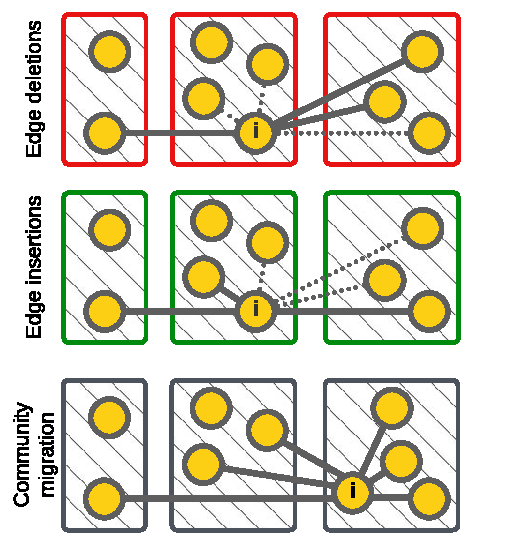
\includegraphics[width=0.3\linewidth]{out/about-cases-naive.pdf}
  % }
  \subfigure[Delta-screening (DS)]{
    \label{fig:about-cases--delta}
    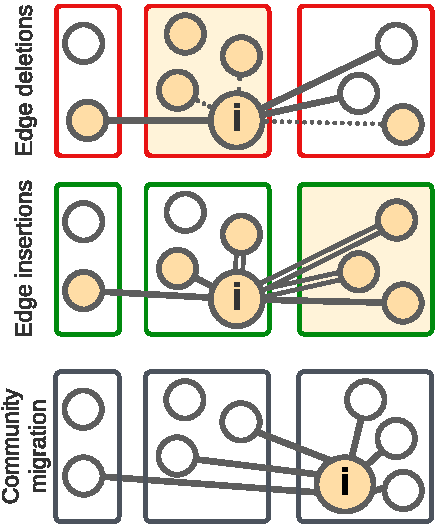
\includegraphics[width=0.468\linewidth]{out/about-cases-delta.pdf}
  }
  \subfigure[Dynamic Frontier (DF)]{
    \label{fig:about-cases--frontier}
    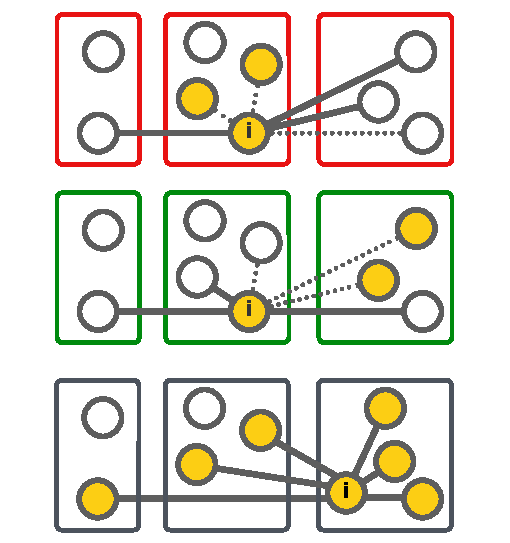
\includegraphics[width=0.43\linewidth]{out/about-cases-frontier.pdf}
  } \\[-1ex]
  \caption{Illustration of \textit{Delta-screening (DS)} \cite{com-zarayeneh21} and \textit{Dynamic Frontier (DF)} approaches \cite{sahu2024shared}, in the presence of edge deletions and insertions, represented with dotted lines and doubled lines, respectively. Vertices identified as affected (initial) by each approach are highlighted in brown, and entire communities marked as affected are depicted in light brown.}
  \label{fig:about-cases}
\end{figure}


\paragraph{Initial marking of affected vertices upon edge deletion/insertion}

For edge deletions between vertices belonging to the same community and edge insertions between vertices belonging to different communities, we mark the source vertex $i$ as affected, as shown with vertices highlighted in yellow, in Figure \ref{fig:about-cases--frontier}. Note that batch updates are undirected, so we effectively mark both the endpoints $i$ and $j$. Edge deletions between vertices lying across communities and edge insertions for vertices lying within the same community are ignored (for reasons stated before, in Section \ref{sec:delta-screening}).

\paragraph{Incremental marking of affected vertices on vertex migration to another community}

When a vertex $i$ changes its community during the community detection algorithm (shown by moving $i$ from its original community in the center to its new community on the right), we mark all its neighbor vertices $j \in J_i$ as affected, as shown in Figure \ref{fig:about-cases--frontier} (highlighted in yellow), and mark $i$ as not affected. To minimize unnecessary computation, we also mark an affected vertex $i$ as not affected even if $i$ does not change its community. We call this as the vertex pruning optimization \cite{com-ozaki16, com-ryu16, com-shi21, com-zhang21}. The process is akin to a graph traversal and continues until the community assignments of the vertices have converged.

\paragraph{Application to the first pass of Leiden algorithm}

We apply the DF approach to the first pass of Leiden algorithm\ignore{(see line \ref{alg:leiden--remark-pass} in Algorithm \ref{alg:leiden})}, as with the DS approach. In subsequent passes\ignore{, if the aggregation tolerance condition is not met (line \ref{alg:leiden--aggregation-tolerance} in Algorithm \ref{alg:leiden}),} all super-vertices are marked as affected and processed according to Leiden. This takes less than $14\%$ of total time, so we don't use the DF approach to find affected super-vertices.\ignore{The tolerance condition only fails in the case of large batch updates.} The psuedocode for our parallel DF Leiden is given in Algorithm \ref{alg:frontier}, with its explanation in Section \ref{sec:our-frontier}. Similar to our parallel ND/DS Leiden, it utilizes\ignore{weighted-degrees of vertices and total edge weights of communities as} auxiliary information.




\subsection{Utilizing Auxiliary information}
\label{sec:auxiliary}

We note that computing the weighted-degree of each vertex $K^t$ and the total edge weight of each community $\Sigma^t$ incurs considerable runtime, in comparison to the time required for the local-moving and aggregation phases of the Leiden algorithm\ignore{to converge, especially for small batch updates}. It would be more efficient to incrementally update the previous weighted-degrees of vertices $K^{t-1}$ and total edge weights of communities $\Sigma^{t-1}$ by taking into account edge deletions $\Delta^{t-}$ and insertions $\Delta^{t+}$ within the batch update, instead of recomputing from scratch. We refer to $K^t$ and $\Sigma^t$ (and $K^{t-1}$, $\Sigma^{t-1}$) as auxiliary information as they must be maintained by the dynamic algorithm, but do not represent the output of the algorithm. Figure \ref{fig:about-auxiliary} illustrates this concept.

In Figure \ref{fig:adjust-auxiliary}, we present the mean speedup observed for ND, DS, and DF Leiden when making use of auxiliary information $K^{t-1}$ and $\Sigma^{t-1}$, in contrast to the same dynamic algorithm when calculating from scratch. This is done on graphs from Table \ref{tab:dataset-large} with random batch updates of size $10^{-7} |E|$ to $0.1 |E|$, consisting of $80\%$ edge insertions and $20\%$ edge deletions, to simulate realistic dynamic graph updates. Results indicate that employing auxiliary information enables ND, DS, and DF Leiden to achieve average speedups of $11.8\times$, $2.9\times$, and $48.5\times$, respectively. Moreover, DF Leiden achieves remarkable speedups, reaching up to $107\times$ for smaller batch sizes. Incrementally updating $K^{t-1}$ and $\Sigma^{t-1}$ to obtain $K^t$ and $\Sigma^t$, thus, significantly speeds up DF Leiden. To the best of our knowledge, none of the existing dynamic algorithms for Leiden algorithm make such use of auxiliary information.

\begin{figure}[hbtp]
  \centering
  \subfigure{
    \label{fig:about-auxiliary--with}
    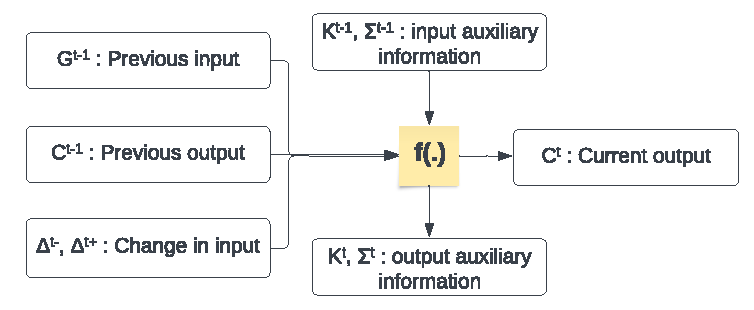
\includegraphics[width=0.98\linewidth]{out/about-auxiliary-with.pdf}
  } \\[-2ex]
  \caption{A dynamic community detection algorithm $f(.)$ takes as input the previous graph $G^{t-1}$, community memberships $C^{t-1}$, and the batch update $\Delta^{t-}$, $\Delta^{t+}$, and produces the updated community memberships $C^t$. However, it may also consider additional information such as the weighted degrees of vertices $K^{t-1}$ and the total edge weights of communities $\Sigma^{t-1}$ as auxiliary information, and yield updated auxiliary information $K^t$, $\Sigma^t$ \cite{sahu2024dflouvain}.}
  \label{fig:about-auxiliary}
\end{figure}





\subsection{Our DF Leiden implementation}
\label{sec:our-frontier}

Algorithm \ref{alg:frontier} shows the psuedocode of our Parallel Dynamic Frontier (DF) Leiden. It takes as input the previous $G^{t-1}$ and current graph snapshot $G^t$, edge deletions $\Delta^{t-}$ and insertions $\Delta^{t+}$ in the batch update, the previous community assignments $C^{t-1}$ for each vertex, the previous weighted-degrees $K^{t-1}$ of vertices, and the previous total edge weights $\Sigma^{t-1}$ of communities. It returns the updated community memberships $C^t$ of vertices, weighted-degrees $K^t$, and total edge weights $\Sigma^t$ of communities.

\begin{algorithm}[hbtp]
\caption{Our Parallel \textit{Dynamic Frontier (DF)} Leiden \cite{sahu2024dflouvain}.}
\label{alg:frontier}
\begin{algorithmic}[1]
\Require{$G^t(V^t, E^t)$: Current/updated input graph}
\Require{$\Delta^{t-}, \Delta^{t+}$: Edge deletions and insertions (batch update)}
\Require{$C^{t-1}, C^t$: Previous, current community of each vertex}
\Require{$K^{t-1}, K^t$: Previous, current weighted-degree of vertices}
\Require{$\Sigma^{t-1}, \Sigma^t$: Previous, current total edge weight of communities}
\Ensure{$\delta V$: Flag vector indicating if each vertex is affected}
\Ensure{$isAffected(i)$: Is vertex $i$ is marked as affected?}
\Ensure{$inAffectedRange(i)$: Can $i$ be incrementally marked?}
\Ensure{$onChange(i)$: What happens if $i$ changes its community?}
\Ensure{$F$: Lambda functions passed to parallel Leiden (Alg. \ref{alg:leiden})}

\Statex

\Function{dynamicFrontier}{$G^t, \Delta^{t-}, \Delta^{t+}, C^{t-1}, K^{t-1}, \Sigma^{t-1}$}
  \State $\rhd$ Mark initial affected vertices
  \ForAll{$(i, j) \in \Delta^{t-}$ \textbf{in parallel}} \label{alg:frontier--loopdel-begin}
    \If{$C^{t-1}[i] = C^{t-1}[j]$} $\delta V[i] \gets 1$
    \EndIf
  \EndFor \label{alg:frontier--loopdel-end}
  \ForAll{$(i, j, w) \in \Delta^{t+}$ \textbf{in parallel}} \label{alg:frontier--loopins-begin}
    \If{$C^{t-1}[i] \neq C^{t-1}[j]$} $\delta V[i] \gets 1$
    \EndIf
  \EndFor \label{alg:frontier--loopins-end}
  \Function{isAffected}{$i$} \label{alg:frontier--isaff-begin}
    \Return{$\delta V[i]$}
  \EndFunction \label{alg:frontier--isaff-end}
  \Function{inAffectedRange}{$i$} \label{alg:frontier--isaffrng-begin}
    \Return{$1$}
  \EndFunction \label{alg:frontier--isaffrng-end}
  \Function{onChange}{$i$} \label{alg:frontier--onchg-begin}
    \ForAll{$j \in G^t.neighbors(i)$} $\delta V[j] \gets 1$
    \EndFor
  \EndFunction \label{alg:frontier--onchg-end}
  \State $F \gets \{isAffected, inAffectedRange, onChange\}$ \label{alg:frontier--lambdas}
  \State $\rhd$ Use $K^{t-1}$, $\Sigma^{t-1}$ as auxiliary information (Alg. \ref{alg:update})
  \State $\{K^t, \Sigma^t\} \gets updateWeights(G^t, \Delta^{t-}, \Delta^{t+}, C^{t-1}, K^{t-1}, \Sigma^{t-1})$\label{alg:frontier--auxiliary}
  \State $\rhd$ Obtain updated communities (Alg. \ref{alg:leiden})
  \State $C^t \gets leiden(G^t, C^{t-1}, K^t, \Sigma^t, F)$ \label{alg:frontier--leiden}
  \Return{$\{C^t, K^t, \Sigma^t\}$} \label{alg:frontier--return}
\EndFunction
\end{algorithmic}
\end{algorithm}


In the algorithm, we first identify an initial set of affected vertices, whose communities may directly change due to the batch updates, by marking them in the flag vector $\delta V$. We do this by marking the endpoints of edge deletions $\Delta^{t-}$ which lie in the same community (lines \ref{alg:frontier--loopdel-begin}-\ref{alg:frontier--loopdel-end}), and by marking the endpoints of edge insertions $\Delta^{t+}$ which lie is disjoint communities (lines \ref{alg:frontier--loopins-begin}-\ref{alg:frontier--loopins-end}). We then define three lambda functions for the Leiden algorithm, \texttt{isAffected()} (lines \ref{alg:frontier--isaff-begin}-\ref{alg:frontier--isaff-end}), \texttt{inAffectedRange()} (lines \ref{alg:frontier--isaffrng-begin}-\ref{alg:frontier--isaffrng-end}), and \texttt{onChange()} (lines \ref{alg:frontier--onchg-begin}-\ref{alg:frontier--onchg-end}), which indicate that a set of vertices are (initially) marked as affected, that all vertices in the graph can be incrementally marked as affected, and that the neighbors of a vertex are marked as affected if it changes its community membership, respectively. Note that the set of affected vertices will expand automatically due to vertex pruning optimization used in our Parallel Leiden algorithm (Algorithm \ref{alg:leiden}). Thus, \texttt{onChange()} reflects what the DF approach would do in the absence of vertex pruning. Further, unlike existing approaches, we leverage $K^{t-1}$ and $\Sigma^{t-1}$, alongside the batch updates $\Delta^{t-}$ and $\Delta^{t+}$, to efficiently compute $K^t$ and $\Sigma^t$ required for the local-moving phase of the Leiden algorithm (line \ref{alg:frontier--auxiliary}). These lambda functions and the total vertex/edge weights are then utilized to execute the Leiden algorithm and obtain the updated community assignments $C^t$ (line \ref{alg:frontier--leiden}). Finally, we return $C^t$, alongside $K^t$ and $\Sigma^t$\ignore{, serving as the updated auxiliary information} (line \ref{alg:frontier--return}).
